%=================================================================
\section{Introduction}\label{sec-intro}

This project required to build a model that predicts the total ride duration of taxi trips in New York City. The primary dataset is one released by the NYC Taxi and Limousine Commission, which includes pickup time, geo-coordinates, number of passengers, picktime and dropoff time, and several other variables.
\\In this section, The train data which we have 1458644 Rows and 11 columns. The test data which we have 625134 Rows and 9 columns.
\\We built the linearregression model, using distance to predict the trip duration and test.

\section{Data ETL} 

\begin{itemize}
	\item
	%\emph{New York City Taxi Trip Duration Prediction}
     Read train data and test data from csv files.
	
\end{itemize} 


%%%%%%%%%% -------------------------------------------------------------------- %%%%%%%%%%
{
	\begin{itemize}
		\item
		%\emph{New York City Taxi Trip Duration Prediction}
		 After we read, clearn the data and check NAs, The train data which we have 1458644 Rows and 11 columns. The test data which we have 625134 Rows and 9 columns.We built the linearregression model, using distance to predict the trip duration and test.
		
		\item
		Data Types
	\end{itemize} 
	
	\bigskip 
	\begin{tabular}{ l | l }
		\toprule
		Attribute     &  Description          \\
		\midrule
		vendor id               & a code indicating the provider associated with the trip record\\
		pickup datetime      &  date and time when the meter was engaged  \\
		dropoff datetime     &  date and time when the meter was disengaged  \\
		pickup longitude     &  the longitude where the meter was engaged\\ 
		pickup latitude        &  the latitude where the meter was engaged\\ 
		dropoff longitude    & the longitude where the meter was disengaged\\ 
		dropoff latitude       & the latitude where the meter was disengaged\\ 
		store and fwd flag   &  Y=store and forward; N=not a store and forward trip\\
		trip duration           & duration of the trip in seconds\\
		
		\bottomrule
	\end{tabular}	
	
}
%%%%%%%%%% -------------------------------------------------------------------- %%%%%%%%%%



%%%%%%%%%% -------------------------------------------------------------------- %%%%%%%%%%
\section{Knowledge Discovery} 
Visualise Data:

\begin{itemize}
\item
Distance characteristic analysis
\item
Distance characteristic analysis
\end{itemize} 

%%%%%%%%%% -------------------------------------------------------------------- %%%%%%%%%%
{
	\vspace{0.5cm} 
	\begin{flushleft}
		\centering
		\selectcolormodel{rgb}
		%  \missingfigure{Testing a long text string.}
		\includegraphics[width=0.5\textwidth]{figures//pe7.eps}\\
		%  \caption{The amount rented at different times of the day} \label{framework}
	\end{flushleft}
	
	\begin{flushleft}
		\centering
		\selectcolormodel{rgb}
		%  \missingfigure{Testing a long text string.}
		\includegraphics[width=0.5\textwidth]{figures//pe8.eps}\\
		%  \caption{The amount rented at different times of the day} \label{framework}
	\end{flushleft}
}
%%%%%%%%%% -------------------------------------------------------------------- %%%%%%%%%%

\section{Select features and gropby data} 
{
	\begin{description}
		\item
		Select ’trip duration’ and ’distance’ as features, groupby data to train data and test
		data in the train dataframe, set 0 to 150 as train data, 150 to 180 as test data,
		named as train and test
	\end{description}
	\vspace{-0.8cm}
	\begin{flushleft}
		\centering
		\selectcolormodel{rgb}
		%  \missingfigure{Testing a long text string.}
		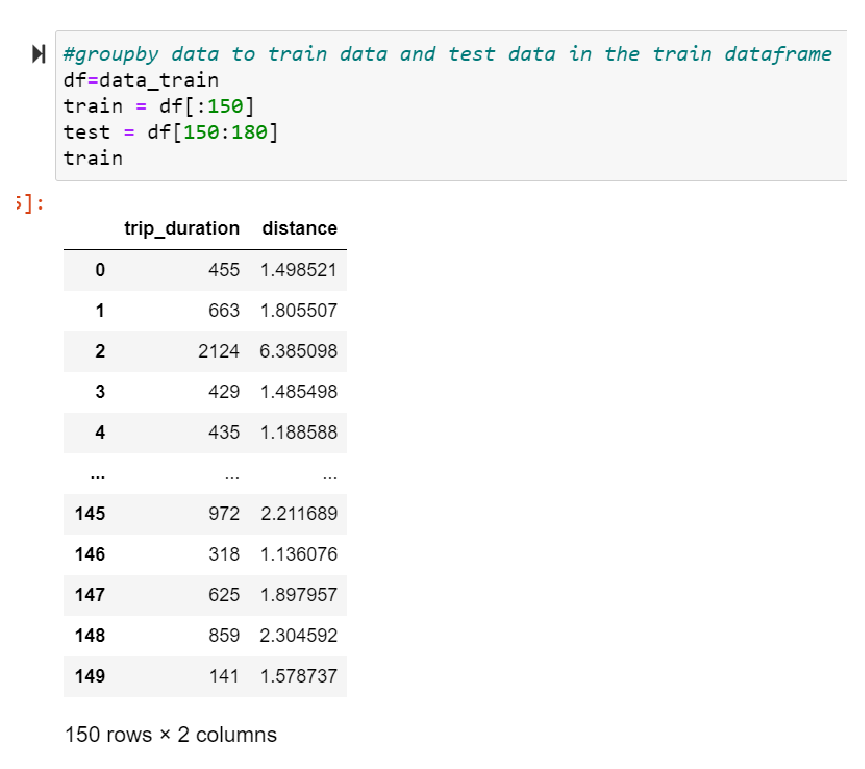
\includegraphics[width=0.7\textwidth]{figures//pe13.eps}\\
		%\caption{Correlation rank} \label{framework}
	\end{flushleft}
	
}
%%%%%%%%%% -------------------------------------------------------------------- %%%%%%%%%%


%%%%%%%%%% -------------------------------------------------------------------- %%%%%%%%%%
\section{Built Modeling and Predict Result}
{
	\begin{description}
		\item[Model:] LinearRegression Model
		
	\end{description}
	\vspace{.5cm}
	\begin{description}
		\item[RSMLE:] 4.616529350404572
		
	\end{description}
	
}
%%%%%%%%%% -------------------------------------------------------------------- %%%%%%%%%%




%%%%%%%%%% -------------------------------------------------------------------- %%%%%%%%%%
\section{Visualize Predict Result}

%%%%%%%%%% -------------------------------------------------------------------- %%%%%%%%%%

{
	\begin{itemize}
		\item
		Trip Duration Visualize Predict Result
	\end{itemize} 
	\vspace{0.5cm} 
	\begin{flushleft}
		\centering
		\selectcolormodel{rgb}
		%  \missingfigure{Testing a long text string.}
		\includegraphics[width=0.7\textwidth]{figures//pe15.eps}\\
		%  \caption{The amount rented at different times of the day} \label{framework}
	\end{flushleft}
	
}
%%%%%%%%%% -------------------------------------------------------------------- %%%%%%%%%%

\section{Conclusions} \label{sec-conclusions}

The Propose of this project which is to find the data features, select the attruibuates to built the linearregression model, find the best parameter using distance data to predict the trip duration and test.But , from the chart we can see the model is not very good, maybe we an explore other model to improve the accuracy.



